\chapter{RELATED THEORY}

\section{Decentralization}
Decentralization refers to the distribution of authority, control, and decision-making away from a central authority. In the context of digital platforms, decentralization allows users to maintain control over their data and interactions, fostering a more democratic and resilient online environment. This approach contrasts with traditional centralized systems, where a single entity governs all operations and data management. 
\begin{figure}[h]
  \centering
    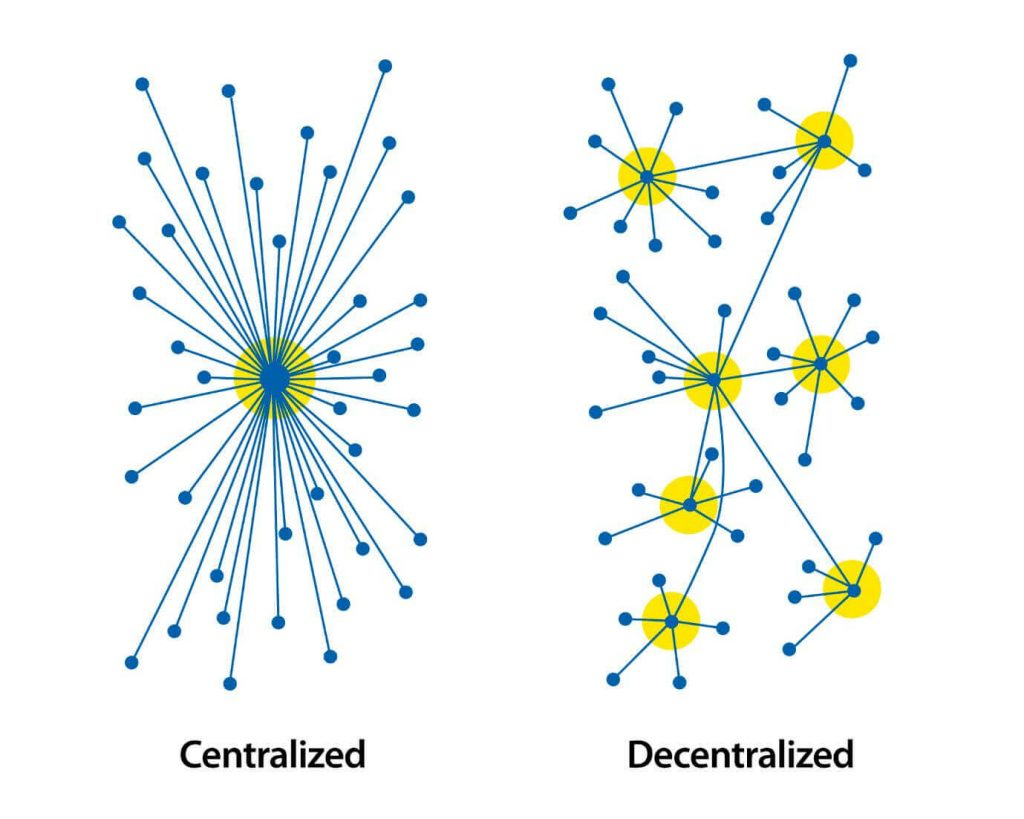
\includegraphics[width=0.75\textwidth]{Graphics/centvsdecent.jpg} % Adjust the width as needed
    \caption{The structure of a centralized network compared to a decentralized network.}
    \label{fig:example}
\end{figure}
\section{Federation}
Federation is a model that enables different systems or organizations to interoperate while maintaining their independence. In social media, a federated approach allows users from different platforms to communicate and share content seamlessly, creating a more interconnected online community. This is achieved through protocols that facilitate data exchange and interaction across diverse platforms.

\section{Scientific Typesetting}
Scientific typesetting involves the formatting of mathematical and scientific content for clarity and precision. It is essential for effectively communicating complex ideas in academic and research contexts. Proper typesetting ensures that equations, symbols, and notations are presented in a way that is easily understandable and visually appealing. The prime example of a Scientific Typesetting is LaTeX but there are alternatives like AsciiMath and Typst.

\section{ActivityPub Protocol}
ActivityPub is a decentralized social networking protocol standardized by the World Wide Web Consortium (W3C) \cite{ActivityPub}. It provides a client-to-server API for creating, updating, and deleting content, as well as a server-to-server API for delivering notifications and content between different servers. 

The federation model offers several key advantages over centralized systems, such as resilience (no single point of failure as the network operates across multiple independent servers), data sovereignty (each instance maintains control over its users' data and policies), interoperability (users can communicate across instances using standardized protocols), and scalability (the network can grow organically as new instances join the federation).
\begin{figure}[h]
  \centering
    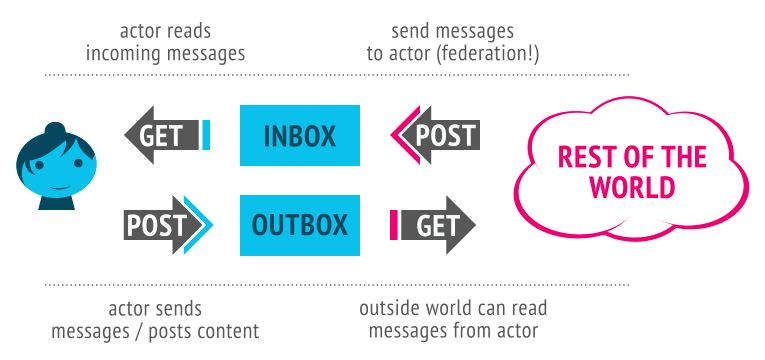
\includegraphics[width=0.95\textwidth]{Graphics/activitypubexample.png} % Adjust the width as needed
    \caption{Communication using ActivityPub Protocol.}
    \label{fig:example}
\end{figure}

 The protocol is built on several key concepts:

\begin{itemize}
  \item \textbf{Actors} which represent users, groups, or applications that can send and receive activities.
  \item \textbf{Activities} which describe actions that actors take.
  \item \textbf{Objects} which represent the content being acted upon.
\end{itemize}

